\documentclass[twocolumn, 10pt]{book}
\setlength\textwidth{6.875in}
\setlength\textheight{8.5in}
% set both margins to 2.5 pc
\setlength{\oddsidemargin}{-0.1875in}% 1 - (8.5 - 6.875)/2
\setlength{\evensidemargin}{-0.1875in}
\setlength{\marginparwidth}{0pc}
\setlength{\marginparsep}{0pc}%
\setlength{\footskip}{37pt}%
\setlength{\columnsep}{0.25in}
%\setlength{\columnwidth}{3.28125in}% (6.875 - 0.3125)/2 = 3.28125in
\setlength{\parindent}{1pc}
\newcommand{\myMargin}{1.00in}
\setlength{\topmargin}{0pt} 
\setlength{\headheight}{22pt}
\setlength{\headsep}{20pt}
\usepackage[top=\myMargin, left=\myMargin, right=\myMargin, bottom=\myMargin]{geometry}
\usepackage{epsfig,graphicx}
\usepackage{palatino}
\usepackage{fancybox}
\usepackage{hyperref}
\usepackage[svgnames]{xcolor}
\usepackage[procnames]{listings}

% "define" Scala
\usepackage[T1]{fontenc}  
\usepackage[scaled=0.82]{beramono}  
\usepackage{microtype} 

\sbox0{\small\ttfamily A}
\edef\mybasewidth{\the\wd0 }

\lstdefinelanguage{scala}{
  morekeywords={abstract,case,catch,class,def,%
    do,else,extends,false,final,finally,%
    for,if,implicit,import,match,mixin,%
    new,null,object,override,package,%
    private,protected,requires,return,sealed,%
    super,this,throw,trait,true,try,%
    type,val,var,while,with,yield},
  sensitive=true,
  morecomment=[l]{//},
  morecomment=[n]{/*}{*/},
  morestring=[b]",
  morestring=[b]',
  morestring=[b]"""
}

\usepackage{color}
\definecolor{dkgreen}{rgb}{0,0.6,0}
\definecolor{gray}{rgb}{0.5,0.5,0.5}
\definecolor{mauve}{rgb}{0.58,0,0.82}

% Default settings for code listings
\lstset{frame=tb,
  language=scala,
  aboveskip=3mm,
  belowskip=3mm,
  showstringspaces=false,
  columns=fixed, % basewidth=\mybasewidth,
  basicstyle={\small\ttfamily},
  numbers=none,
  numberstyle=\footnotesize\color{gray},
  % identifierstyle=\color{red},
  keywordstyle=\color{blue},
  commentstyle=\color{dkgreen},
  stringstyle=\color{mauve},
  frame=single,
  breaklines=true,
  breakatwhitespace=true,
  procnamekeys={def, val, var, class, trait, object, extends},
  procnamestyle=\ttfamily\color{red},
  tabsize=2
}

\lstnewenvironment{scala}[1][]
{\lstset{language=scala,#1}}
{}
\lstnewenvironment{cpp}[1][]
{\lstset{language=C++,#1}}
{}
\lstnewenvironment{bash}[1][]
{\lstset{language=bash,#1}}
{}
\lstnewenvironment{verilog}[1][]
{\lstset{language=verilog,#1}}
{}



\lstset{basicstyle={\footnotesize\ttfamily}}

\newenvironment{commentary}
{ \vspace{-0.1in}
  \begin{quotation}
  \noindent
  \small \em
  \rule{\linewidth}{1pt}\\
}
{
  \end{quotation}
}

\title{Getting Started with Chisel}
\author{Jonathan Bachrach, Vincent Lee \\
EECS Department, UC Berkeley\\
{\tt  \{jrb\}@eecs.berkeley.edu}
}
\date{\today}

\newenvironment{example}{\VerbatimEnvironment\begin{footnotesize}\begin{Verbatim}}{\end{Verbatim}\end{footnotesize}}
\newcommand{\kode}[1]{\begin{footnotesize}{\tt #1}\end{footnotesize}}

\definecolor{RED}{rgb}{1,0,0}
\def\red#1{{\color{red}#1}}
\def\problem#1{{\red{#1 Problem}}}
\def\code#1{{\tt #1}}

\def\note#1{\noindent{\bf [Note: #1]}}
%\def\note#1{}

\begin{document}
\maketitle{}

\chapter{Chisel Installation}
\section{Introduction}

This chapter is an installation guide for {\em Chisel} (Constructing
Hardware In a Scala Embedded Language) and is intended to prepare your system for subsequent tutorials.  Chisel is a hardware
construction language embedded in the high-level programming language
Scala.

\subsection{Development Tool Installation}

If you are running Mac or a variant of Linux, you will need to install the appropriate tools for your OS, which are described in the following sections:

\subsubsection{MacOSX}

\begin{enumerate}
\item Install XCODE, including console tools.
\end{enumerate}

\subsubsection{Linux}

Install the following packages:

\begin{enumerate}
\item \verb|g++-4.8|
\item \verb+openjdk-7-jre+
\end{enumerate}

\noindent
using

\begin{bash}
sudo apt-get install
\end{bash}

\section{Setting Up the Tutorial}

In subsequent tutorials, you will be using the files distributed in the chisel-tutorial repository. To obtain these tutorials files, \verb+cd+ to the directory = \verb+$DIR+ where you want to place the Chisel tutorial and type:

\begin{bash}
cd $DIR
git clone https://github.com/ucb-bar/chisel-tutorial.git
\end{bash}

\noindent
Your copy of the Chisel Tutorial repository will then be in \verb+$DIR/chisel-tutorial+.  Define this as a variable in your bash environment named \verb+$TUT_DIR+.

This is the Chisel tutorial directory structure you should see, which is explained more in the next tutorial:

\begin{bash}
chisel-tutorial/  
  Makefile
  examples/
    Makefile
    build.sbt
    Accumulator.scala ...
  problems/
    Makefile
    build.sbt
    Counter.scala ...
  solutions/
    Makefile
    build.sbt
    Counter.scala ...
\end{bash}

\noindent 

The following tutorials will explain features of Chisel by presenting source code examples.  The repository is split into examples, problems, and solutions, where the problems have some piece of the design for you to fill out and where the examples and solutions are meant to be complete designs that should pass the given tests.  In order to run either, you simply need to change directory into the appropriate subdirectory and type \verb+make+ of the particular lesson name. We will use the repository to first test out if your machine is set up to use Chisel.

To test your Chisel distribution and verify that your system contains all the correct tools, run the following commands:

\begin{bash}
cd $TUT_DIR/examples
make Parity.out
\end{bash}

This will run a test build and will take a minute before it completes. If your system is set up correctly, you should see a messsage \verb+[success]+ followed by the total time of the run, and date and time of completion. If you see a success than your system has been set up correctly and you can continute to the next tutorial where we will explain more about the basics of Chisel.

\section{The Tutorials}

For these tutorials, we assume basic knowledge of digital circuits and blocks. 
Tutorial 1 will guide you through a quick compilation of the emulator and Verilog generation, and explain some basic constructs such as register and combinational logic.
Tutorial 2 will explain the basics of Chisel.
Tutorial 3 will explain how to use basic primitive types and logical operations that are used in Chisel and how to use them in context of several examples. 
Tutorial 4 will explain how to instantiate components and apply parametrization. 
Tutorial 5 will explain how to use the Chisel test harness. 
Tutorial 6 will explain how to set up your own Chisel project and how to build it.
Tutorial 7 will revisit conditional register updates and explain how to construct memories.
Finally, tutorial 8 will introduce how to use Scala constructs such as \verb+if...else+ and \verb+for+ loops.

Along the way there are assignments highlighted with \red{red} titles.  
These assignments are built around files in the tutorial problems directory.
In order to check successful completion of the entire set of getting started assignments run:
\begin{bash}
cd $TUT_DIR/problems
make getting-started
\end{bash}

\noindent
until no error appears.

The following set of tutorials were written using the build settings Scala version 2.11 and Chisel version 2.2.


\chapter{The Basics}
\subsection{The Chisel Directory Structure}

Once you have acquired the tutorial files you should see the following Chisel tutorial directory structure under \verb+$TUT_DIR+:

\begin{bash}
chisel-tutorial/  
  Makefile
  examples/   # chisel examples
    Makefile  # for running examples
    build.sbt # project description
    Accumulator.scala ...
  problems/   # skeletal files for tutorial problems
    Makefile  # for running / testing problems
    build.sbt # project description
    Counter.scala ...
  solutions/  # solutions to problems
    Makefile  # for running solutions
    build.sbt # project description
    Counter.scala ...
\end{bash}

Chisel source files are distributed between \verb+examples+, \verb+problems+, and \verb+solutions+ directories.
The tutorial contains the files that you will be modifying under \verb+problems/+ while the \verb+solutions/+ folder contains the reference implementations for each of the problems.  Finally, \verb+examples/+ contains source to the complete examples given in this tutorial.

Finally, the \verb+build.sbt+ files contain the build configuration information used to specify what version of Chisel to make your project with.

\section{Running Your First Chisel Build}

In this section, we explain how to run your first build to explore what Chisel has to offer. We will go through a simple example for a GCD module and familiarize ourselves with the source files, simulation, and Verilog generation. More comprehensive details will follow in subsequent sections of the tutorial.

\subsection{The Chisel Source Code}

Now that you are more familiar with what your Chisel directory structure contains, let's start by exploring one of the Chisel files. Change directory into the \verb+examples/+ directory and open up the \verb+GCD.scala+ file with your favorite text editor. 

You will notice that file is already filled out for you to perform the well known GCD algorithm and should look like:

\begin{scala}
package TutorialExamples

import Chisel._

class GCD extends Module {
  val io = new Bundle {
    val a  = UInt(INPUT,  16)
    val b  = UInt(INPUT,  16)
    val e  = Bool(INPUT)
    val z  = UInt(OUTPUT, 16)
    val v  = Bool(OUTPUT)
  }
  val x  = Reg(UInt())
  val y  = Reg(UInt())
  when   (x > y) { x := x - y } 
  unless (x > y) { y := y - x }
  when (io.e) { x := io.a; y := io.b }
  io.z := x
  io.v := y === UInt(0)
} ...
\end{scala}

The first thing you will notice is the \verb+import Chisel._+ declaration; this imports the Chisel library files that allow us to leverage Scala as a hardware construction language. After the import declarations you will see the Scala class definition for the Chisel component you are implementing. You can think of this as almost the same thing as a module declaration in Verilog.

Next we see the I/O specification for this component in the \verb+val io = new Bundle{...}+ definition. You will notice that the bundle takes several arguments as part of its construction, each with a specified type (UInt, Bool, etc.), a direction (either INPUT or OUTPUT), and a bit width. If a bit width is not specified, Chisel will infer the appropriate bit width for you (in this case default to 1). The \verb+io+ Bundle is essentially a constructor for the component that we are constructing.

The next section of code performs the actual GCD computation for the module. The register declarations for \verb+x+ and \verb+y+ tell Chisel to treat \verb+x+ and \verb+y+ as a register of type UInt(). 

\begin{scala}
val x = Reg(UInt()) // declares x as UInt register
val y = Reg(UInt()) // declares y as UInt register
\end{scala}

The \verb+when+ statement tells Chisel to perform the operation on a positive clock edge if the condition is true, treating the left hand assignments as synchronous. This is similar to how Verilog uses \verb+always @ (posedge clk)+ to specify synchronous logic.

Finally we see the output assignments for the computation for \verb+io.z+ and \verb+io.v+. One particular thing to notice is that, we do not have to specify the width of \verb+x+ and \verb+y+ in this example. This is because Chisel does the bit width inference for you and sets these values to their appropriate widths based on the computation they are storing.

\subsection{Running the Chisel Simulation}

Now that we are familiar with the Chisel code for the \verb+GCD.scala+ file, let's try to simulate it by generating the C++ models. Change directory into the \verb+$DIR/examples/+ directory. Here you will see one lonely Makefile which we will call with:

\begin{bash}
make GCD.out
\end{bash}

\noindent
This will fire off the Chisel emulator that will run the simulation for the component defined in \verb+GCD.scala+. If the simulation succeeds, you should see some debug output followed by:
\begin{footnotesize}
\begin{bash}
PASSED
[success] Total time: 2 s, completed Feb 28, 2013 \
  8:14:37 PM
\end{bash}
\end{footnotesize}

The debug output is generated by the test harness which composes the second half of the GCD.scala file. We will talk about this more later. In addition to the debug output, the build also creates C++ models which can be used to simulate and debug more complicated designs.

\subsection{Generating the Verilog}

One of the most powerful features of Chisel is its ability to generate FPGA and ASIC Verilog from the Scala sources that you construct. To do this, change directory into the \verb+$DIR/examples/verilog/+ directory and again run:
\begin{bash}
make GCD.v
\end{bash}
This will start the Verilog generation for the GCD Chisel file. When the Verilog generation finishes, you should see a [success] message similar to the one you saw in the emulator and a new \verb+GCD.v+ file. If you open up \verb+GCD.v+, you will find that Chisel has compiled \verb+GCD.scala+ into its equivalent Verilog source.

You will find that the Chisel compiler has generated an equivalent Verilog module that performs the GCD computation.

The Verilog source is roughly divided into three parts:
\begin{enumerate}
\item Module declaration with input and outputs
\item Temporary wire and register declaration used for holding intermediate values
\item Register assignments in \verb+always @ (posedge clk)+
\end{enumerate}

\section{Combinational Logic}

\subsection{The Scala Node: Declaring Wires}

Constructing combinational logic blocks in Chisel is fairly straightforward; when you declare a \verb+val+ in Scala, it creates a node that represents the data that it is assigned to. As long as the value is not assigned to be a register type (explained later), this tells the Chisel compiler to treat the value as wire. Thus any number of these values can be connected and manipulated to produce the value that we want.

Suppose we want to construct a single full adder. A full adder takes two inputs \verb+a+ and \verb+b+, and a carry in \verb+cin+ and produces a \verb+sum+ and carry out \verb+cout+. The Chisel source code for our full adder will look something like:

\begin{scala}
class FullAdder extends Module {
  val io = new Bundle {
    val a    = UInt(INPUT, 1)
    val b    = UInt(INPUT, 1)
    val cin  = UInt(INPUT, 1)
    val sum  = UInt(OUTPUT, 1)
    val cout = UInt(OUTPUT, 1)
  }
  // Generate the sum
  val a_xor_b = io.a ^ io.b
  io.sum := a_xor_b ^ io.cin
  // Generate the carry
  val a_and_b = io.a & io.b
  val b_and_cin = io.b & io.cin
  val a_and_cin = io.a & io.cin
  io.cout := a_and_b | b_and_cin | a_and_cin
}
\end{scala}

\noindent
where \verb+cout+ is defined as a combinational function of inputs \verb+a+, \verb+b+, and \verb+cin+.

You will notice that in order to access the input values from the \verb+io+ bundle, you need to first reference \verb+io+ since the input and output values belong to the \verb+io+ bundle. The |, \&, and \^\ operators correspond to bitwise OR, AND, and XOR operations respectively.

The corresponding wires for each of these values is shown below in Figure~\ref{fig:full-adder}.  You will notice that each \verb+val+ corresponds to exactly one of the wires.

\begin{figure}[ht!]
\centering
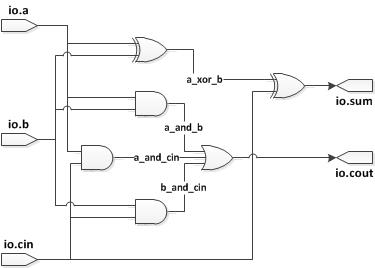
\includegraphics[width=80mm]{figs/Full_Adder.jpg}
\caption{Full Adder Circuit}
\label{fig:full-adder}
\end{figure}


\subsection{Bit Width Inference}

If you don't explicitly specify the width of a value in Chisel, the Chisel compiler will infer the bit width for you based on the inputs that define the value. Notice in the \verb+FullAdder+ definition, the widths for \verb+a_xor_b, a_and_b, b_and_cin,+ and \verb+a_and_cin+ are never specified anywhere. However, based on how the input is computed, Chisel will correctly infer each of these values are one bit wide since each of their inputs are the results of bitwise operations applied to one bit operands.

A quick inspection of the generated Verilog shows these values are indeed one bit wide:

\begin{bash}
module FullAdder(
    input  io_a,
    input  io_b,
    input  io_cin,
    output io_sum,
    output io_cout);

  wire T0;
  wire a_and_cin;
  wire T1;
  wire b_and_cin;
  wire a_and_b;
  wire T2;
  wire a_xor_b;

  assign io_cout = T0;
  assign T0 = T1 | a_and_cin;
  assign a_and_cin = io_a & io_cin;
  assign T1 = a_and_b | b_and_cin;
  assign b_and_cin = io_b & io_cin;
  assign a_and_b = io_a & io_b;
  assign io_sum = T2;
  assign T2 = a_xor_b ^ io_cin;
  assign a_xor_b = io_a ^ io_b;
endmodule
\end{bash}

Suppose we change the widths of the \verb+FullAdder+ to be 2 bits wide each instead such that the Chisel source now looks like:

\begin{scala}
class FullAdder extends Module {
  val io = new Bundle {
    val a    = UInt(INPUT, 2)
    val b    = UInt(INPUT, 2)
    val cin  = UInt(INPUT, 2)
    val sum  = UInt(OUTPUT, 2)
    val cout = UInt(OUTPUT, 2)
  }
  // Generate the sum
  val a_xor_b = io.a ^ io.b
  io.sum := a_xor_b ^ io.cin
  // Generate the carry
  val a_and_b = io.a & io.b
  val b_and_cin = io.b & io.cin
  val a_and_cin = io.a & io.cin
  io.cout := a_and_b | b_and_cin | a_and_cin
}
\end{scala}

As a result, the Chisel compiler should infer each of the intermediate values \verb+a_xor_b, a_and_b, b_and_cin,+ and \verb+a_and_cin+ are two bits wide. An inspection of the Verilog code correctly shows that Chisel inferred each of the intermediate wires in the calculation to be 2 bits wide.

\begin{bash}
module FullAdder(
    input [1:0] io_a,
    input [1:0] io_b,
    input [1:0] io_cin,
    output[1:0] io_sum,
    output[1:0] io_cout);

  wire[1:0] T0;
  wire[1:0] a_and_cin;
  wire[1:0] T1;
  wire[1:0] b_and_cin;
  wire[1:0] a_and_b;
  wire[1:0] T2;
  wire[1:0] a_xor_b;

  assign io_cout = T0;
  assign T0 = T1 | a_and_cin;
  assign a_and_cin = io_a & io_cin;
  assign T1 = a_and_b | b_and_cin;
  assign b_and_cin = io_b & io_cin;
  assign a_and_b = io_a & io_b;
  assign io_sum = T2;
  assign T2 = a_xor_b ^ io_cin;
  assign a_xor_b = io_a ^ io_b;
endmodule
\end{bash}

\section{Using Registers}

Unlike Verilog, specifying a register in Chisel tells the compiler to actually generate a positive edge triggered register. In this section we explore how to instantiate registers in Chisel by constructing a shift register.

In Chisel, when you instantiate a register there are several ways to specify the connection of the input to a register. As shown in the GCD example, you can "declare" the register and assign what it's input is connected to in a \verb+when...+ block or you can simply pass the value that the register is clocking as a parameter to the register.

If you choose to pass a next value to the register on construction using the \verb+next+ named parameter, it will clock the new value every cycle unconditionally:

\begin{scala}
// Clock the new register value on every cycle
val y = io.x
val z = Reg(next = y)
\end{scala}

If we only want to update if certain conditions are met we use a \verb+when+ block to indicate that the registers are only updated when the condition is satisfied:

\begin{scala}
// Clock the new register value when the condition a > b
val x = Reg(UInt())
when (a > b) { x := y }
.elsewhen ( b > a) {x := z}
.otherwise { x := w}
\end{scala}

It is important to note that when using the conditional method, the values getting assigned to the input of the register match the type and bitwidth of the register you declared. In the unconditional register assignment, you do not need to do this as Chisel will infer the type and width from the type and width of the input value.

The following sections show how these can be used to construct a shift register.

\subsection{Unconditional Register Update}

Suppose we want to construct a basic 4 bit shift register that takes a serial input \verb+in+ and generates a serial output \verb+out+. For this first example we won't worry about a parallel load signal and will assume the shift register is always enabled. We also will forget about the register reset signal.

If we instantiate and connect each of these 4 registers explicitly, our Chisel code will look something like:

\begin{scala}
class ShiftRegister extends Module {
  val io = new Bundle {
    val in  = UInt(INPUT, 1)
    val out = UInt(OUTPUT, 1)
  }
  val r0 = Reg(next = io.in)
  val r1 = Reg(next = r0)
  val r2 = Reg(next = r1)
  val r3 = Reg(next = r2)
  io.out := r3
}
\end{scala}

If we take a look at the generated Verilog, we will see that Chisel did indeed map our design to a shift register. One thing to notice is that the clock signal and reset signals are implicitly attached to our design.

\begin{bash}
module ShiftRegister(input clk, input reset,
    input  io_in,
    output io_out);

  reg[0:0] r3;
  reg[0:0] r2;
  reg[0:0] r1;
  reg[0:0] r0;

  assign io_out = r3;
  always @(posedge clk) begin
    r3 <= r2;
    r2 <= r1;
    r1 <= r0;
    r0 <= io_in;
  end
endmodule
\end{bash}

\subsection{Conditional Register Update}

As mentioned earlier, Chisel allows you to conditionally update a register (use an enable signal) using the \verb+when+, \verb+.elsewhen+, \verb+.otherwise+ block. Suppose we add an enable signal to our shift register, that allows us to control whether data is shift in and out on a given cycle depending on an \verb+enable+ input signal. The new shift register now looks like:

\begin{scala}
class ShiftRegister extends Module {
  val io = new Bundle {
    val in     = UInt(INPUT, 1)
    val enable = Bool(INPUT)
    val out    = UInt(OUTPUT, 1)
  }

  val r0 = Reg(UInt())
  val r1 = Reg(UInt())
  val r2 = Reg(UInt())
  val r3 = Reg(UInt())

  when (io.enable) {
    r0 := io.in
    r1 := r0
    r2 := r1
    r3 := r2
  }
  io.out := r3
}
\end{scala}

Notice that it is not necessary to specify an \verb+.otherwise+ condition as Chisel will correctly infer that the old register value should be preserved otherwise.

\subsection{Register Reset}

Chisel allows you to specify a synchronous reset to a certain value by specifying an additional parameter when you first declare them. In our shift register, let's add a reset capability that resets all the register values to zero synchronously. To do this we need to provide our register declarations a little more information using the \verb+init+ parameter with what value we want on a synchronous reset:

\begin{scala}
class ShiftRegister extends Module {
  val io = new Bundle {
    val in     = UInt(INPUT, 1)
    val enable = Bool(INPUT)
    val out    = UInt(OUTPUT, 1)
  }
  // Register reset to zero
  val r0 = Reg(init = UInt(0, width = 1))
  val r1 = Reg(init = UInt(0, width = 1))
  val r2 = Reg(init = UInt(0, width = 1))
  val r3 = Reg(init = UInt(0, width = 1))
  when (io.enable) {
    r0 := io.in
    r1 := r0
    r2 := r1
    r3 := r2
  }
  io.out := r3
}
\end{scala}

Notice that reset value can actually be any value, simply replace the zeros and width to appropriate values.

Chisel also has an implict global \verb+reset+ signal that you can use in a \verb+when+ block. The reset signal is conveniently called \verb+reset+ and does not have to be declared. The shift register using this implict global reset now looks like:

\begin{scala}
class ShiftRegister extends Module {
  val io = new Bundle {
    val in     = UInt(INPUT, 1)
    val enable = Bool(INPUT)
    val out    = UInt(OUTPUT, 1)
  }
  val r0 = Reg(UInt())
  val r1 = Reg(UInt())
  val r2 = Reg(UInt())
  val r3 = Reg(UInt())
  when(reset) {
    r0 := UInt(0)
    r1 := UInt(0)
    r2 := UInt(0)
    r3 := UInt(0)
  } .elsewhen(io.enable) {
    r0 := io.in
    r1 := r0
    r2 := r1
    r3 := r2
  }
  io.out := r3
}
\end{scala}

This will generate slightly different looking Verilog source code but will still function the same as the previous implementation of the shift register with reset.

\subsection{\problem{Sequential Circuit}}

The following exercises can be found in your
\verb+$TUT_DIR/problems/+ folder. You will find that some parts of
the tutorial files have been completed for you and the section that
you need to will need to complete is indicated in the file. The
solutions to each of these exercises can be found in the
\verb+$TUT_DIR/solutions/+ folder.

The first tutorial problem is to write write a sequential circuit that sums \verb+in+ values. 
You can find the template in \verb+$TUT_DIR/problems/Accumulator.scala+ including a stubbed out version of the circuit:
\begin{scala}
class Accumulator extends Module {
  val io = new Bundle {
    val in  = UInt(INPUT, 1)
    val out = UInt(OUTPUT, 8)
  }

  // flush this out ...

  io.out := UInt(0)
}
\end{scala}

\noindent
and a complete tester that confirms that you have successfully designed the circuit.  Run 

\begin{bash}
make Accumulator.out
\end{bash}

\noindent 
until your circuit passes the tests.


%\subsection{Creating a Two Input Multiplexor}
%
%<IS THIS EVEN A GOOD IDEA BECAUSE THEY DON'T REALLY KNOW ANYTHING YET>
%
%\subsection{Creating a Simple FIFO}
%
%<IS THIS EVEN A GOOD IDEA BECAUSE THEY DON'T REALLY KNOW ANYTHING YET>
%


\chapter{Basic Types and Operations}
\section{Chisel Assignments and Reassignments}

When you first define a value in Chisel, we use the \verb+=+ operator in order to tell Chisel to allocate the value for the first time. On every subsequent reassignment to the value, we must use a \verb+:=+ when reassigning the value.

Since we are constructing a digital circuit, the notion of reassignment does not make much sense since connections between circuit nodes only need to be specified once. However, there are some cases when we will need to perform reassignment to a value in Chisel since it is compiled sequentially unlike Verilog. Thus it may be necessary to perform reassignment when a value or connection is not known until later in the Chisel source. 

A simple example of when reassignment is necessary is in the construction of the top level I/O for your module; the values of the output are not immediately known at the time of declaration.

Consider the simple \verb+FullAdder+ circuit from previous tutorial that determines the sum \verb+sum+ and carry out \verb+cout+ given two values \verb+a+ and \verb+b+, and a carry in \verb+cin+.

\begin{scala}
class FullAdder extends Module {
  val io = new Bundle {
    // first definition of io values so use =
    val a    = UInt(INPUT, 1)
    val b    = UInt(INPUT, 1)
    val cin  = UInt(INPUT, 1)
    val sum  = UInt(OUTPUT, 1)
    val cout = UInt(OUTPUT, 1)
  }
  // Generate the sum
  val a_xor_b = io.a ^ io.b
  // Reassignment to io.sum so use :=
  io.sum := a_xor_b ^ io.cin 
  // Generate the carry
  val a_and_b = io.a & io.b
  val b_and_cin = io.b & io.cin
  val a_and_cin = io.a & io.cin
  // reassignment to io.cout so use :=
  io.cout := a_and_b | b_and_cin | a_and_cin
}
\end{scala}

In this example we make sure to use the \verb+:=+ reassignment for the \verb+io.sum+ and \verb+io.cout+ output values because we only know what they're values are later in the code and not at the time of construction of the \verb+io+ Bundle. All other values in this example use the \verb+=+ assignment operator since they need to be created. 

In general, the rule of thumb is to use the reassignment operator \verb+:=+ if the value already has been assigned by the \verb+=+ operator, otherwise the \verb+=+ operator should be used. Note that if you do not use the \verb+=+ or \verb+:=+ operators correctly you will get an error when you try and compile your design.

\section{The Chisel UInt Class}

In the previous examples we have been using the UInt type which is an unsigned integer as the type for all of our values. For many of the basic computations in Chisel the UInt class is sufficient.\footnote{The UInt class definition for Chisel can be found in the /chisel/src/main folder in the compiler source repository, not the chisel-tutorial. You can obtain the Chisel source by cloning https://github.com/ucb-bar/chisel.git} The following example shows some of the commonly used UInt operations in the context of a simple \verb+ALU+\footnote{We ignore overflow and underflow in this example.}:

\begin{scala}
class BasicALU extends Module {
  val io = new Bundle {
    val a      = UInt(INPUT, 4)
    val b      = UInt(INPUT, 4)
    val opcode = UInt(INPUT, 4)
    val output = UInt(OUTPUT, 4)
  }
  io.output := UInt(0) 
  when (io.opcode === UInt(0)) {
    io.output := io.a                   // pass A
  } .elsewhen (io.opcode === UInt(1)) {
    io.output := io.b                   // pass B
  } .elsewhen (io.opcode === UInt(2)) {
    io.output := io.a + UInt(1)         // inc A by 1
  } .elsewhen (io.opcode === UInt(3)) {
    io.output := io.a - UInt(1)         // inc B by 1
  } .elsewhen (io.opcode === UInt(4)) {
    io.output := io.a + UInt(4)         // inc A by 4
  } .elsewhen (io.opcode === UInt(5)) {
    io.output := io.a - UInt(4)         // dec A by 4
  } .elsewhen (io.opcode === UInt(6)) {
    io.output := io.a + io.b            // add A and B
  } .elsewhen (io.opcode === UInt(7)) {
    io.output := io.a - io.b            // sub B from A
  } .elsewhen (io.opcode === UInt(8)) {
    io.output := (io.a < io.b)          // set on A < B
  } .otherwise { 
    io.output := (io.a === io.b)        // set on A == B
  }
}
\end{scala}

You will notice that there are multiple reassignments to \verb+io.output+ inside a \verb+when+ block which indicates that the value of \verb+io.output+ can take many different values depending on the \verb+io.opcode+ in this example. Also notice that in order to specify constants to add to our operands, we must also specify them as a UInt type as UInt operations on different type operands is not allowed.

\begin{scala}
// Specify that 1 is a UInt type
io.output := io.a + UInt(1) 
\end{scala}

A list of commonly used UInt operations is given in the table below:

\begin{center}
\begin{tabular}{| l | l | l | }
\hline
{\bf Operand} & {\bf Operation} & {\bf Output Type} \\ \hline
+ & Add & UInt  \\ \hline
- & Subtract & UInt  \\ \hline
$\ast$ & Multiply & UInt \\ \hline
/ & UInt Divide & UInt \\ \hline
% & Modulo & UInt \\ \hline
\~\ & Bitwise Negation & UInt \\ \hline
\^\ & Bitwise XOR & UInt\\ \hline
\& & Bitwise AND & UInt \\ \hline
 | & Bitwise OR & Bool \\ \hline
=== & Equal & Bool \\ \hline
!= & Not Equal & Bool \\ \hline
> & Greater & Bool \\ \hline
< & Less & Bool \\ \hline
>= & Greater or Equal & Bool \\ \hline
<= & Less or Equal & Bool \\ \hline
\end{tabular}
\end{center}

% Notice that the comparisons for the UInt type give you a Bool type back. In order to be able to assign the output of a comparison to a UInt type, we will need to cast the Bool to a UInt before the assignment. This is shown in the \verb+BasicALU+ example in the \verb+.otherwise+ block:
% 
% \begin{scala}
% io.output :=  (io.a === io.b).toUInt() // set on A == B
% \end{scala}
% 
% If we you do not cast the resulting Bool to a UInt the Chisel compiler will return an error.

\subsection{Bit Extraction}

The UInt class allows you to extract bits based on their index of their representation. Given an \verb+n+ bit wide value \verb+value+ we can extract the bits \verb+x+ through \verb+y+ (n > x > y >= 0) by simply doing the following:

\begin{scala}
// extracts the x through y bits of value
val x_to_y = value(x, y) 
\end{scala}

Note that the higher index is specified first in the argument list when extraction the bits. Also notice that the bits in the UInt are zero indexed so the highest bit that can be extracted from an \verb+n+ bit wide value is \verb+n-1+.

If you just want to extract a single bit from the value, say bit \verb+x+ we simply need to specify a single index instead as follows:
\begin{scala}
// extract the x-th bit from value
val x_of_value = value(x)
\end{scala}

A more concrete example of bit extraction in action is shown below. In this example, based on the value of the offset, we would like to select a byte from a word which is a common operation when loading a byte from word addressed memories:

\begin{scala}
class ByteSelector extends Module {
  val io = new Bundle {
    val in     = UInt(INPUT, 32)
    val offset = UInt(INPUT, 2)
    val out    = UInt(OUTPUT, 8)
  }
  io.out := UInt(0, width = 8)
  when (io.offset === UInt(0)) {
    io.out := io.in(7,0) // pull out lowest byte
  } .elsewhen (io.offset === UInt(1)) {
    io.out := io.in(15,8) // pull out second byte
  } .elsewhen (io.offset === UInt(2)) {
    io.out := io.in(23,16) // pull out third byte
  } .otherwise {
    io.out := io.in(31,24) // pull out highest byte
  }    
}
\end{scala}

\subsection{Bit Concatenation}

Chisel also allows you to easily concatenate bits together using \verb+Cat+. Suppose you have a data bus that you would like to drive with two seperate words \verb+A+ and \verb+B+. In order to concatenate these two values together we simply say:

\begin{scala}
val A = UInt(width = 32)
val B = UInt(width = 32)
val bus = Cat(A, B) // concatenate A and B
\end{scala}

Again, the first argument to \verb+Cat+ will be placed in the high part while the second argument gets the low part of \verb+bus+. Thus for this example bits 0 to 31 of \verb+bus+ correspond to \verb+B+, while bits 32 to 63 correspond to \verb+A+. 

\subsection{\problem{LFSR16}}

In this assignment, write the \verb+LFSR16+ circuit as shown below:

\begin{center}
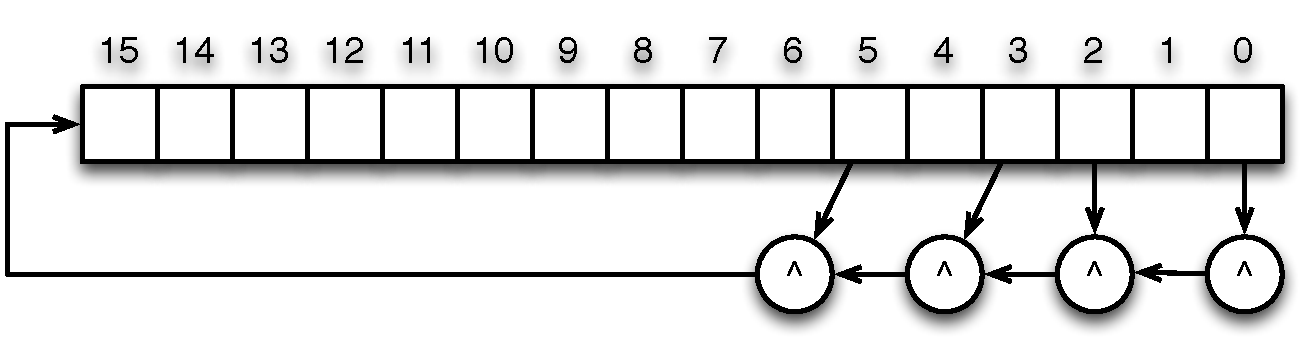
\includegraphics[width=0.9\columnwidth]{../bootcamp/figs/LFSR16.pdf}
\end{center}

\noindent
by filling in the following module:

\begin{scala}
class LFSR16 extends Module {
  val io = new Bundle {
    val inc = Bool(INPUT)
    val out = UInt(OUTPUT, 16)
  }
  // ...
  io.out := UInt(0)
}
\end{scala}

\noindent
found in \verb+$TUT_DIR/problems/LFSR16.scala+.
Make sure to define and initialize an internal register to one and 
update it when \verb+inc+ is asserted.
Use bit concatentation and bit extraction 
in conjunction with the xor operator \verb+^+.  Run 

\begin{bash}
make LFSR16.out
\end{bash}

\noindent 
until your circuit passes the tests.

\subsection{UInt Operation Bit Inference}

Note that for some operations such as addition and multiplication, that number of resulting bits of the computation can be greater than the number of bits for the operands. 

Consider the following example where we multiply two 16 bit numbers \verb+A+ and \verb+B+ together. Note that the product of two 16 bit numbers is at worst 32 bits wide.

\begin{scala}
class HiLoMultiplier() extends Module {
  val io = new Bundle {
    val A  = UInt(INPUT, 16)
    val B  = UInt(INPUT, 16)
    val Hi = UInt(OUTPUT, 16)
    val Lo = UInt(OUTPUT, 16)
  }
  val mult = io.A * io.B
  io.Lo := mult(15, 0)
  io.Hi := mult(31, 16)  
}

\end{scala}

Notice that we never specify the width of the value \verb+mult+ anywhere in the Chisel source. Normally if we performed this in Verilog we would have had to specify the width beforehand. But a look at the generated Verilog for this example shows that Chisel correctly inferred the \verb+mult+ value to be 32 bits wide:

\begin{scala}
module HiLoMultiplier(
    input [15:0] io_A,
    input [15:0] io_B,
    output[15:0] io_Hi,
    output[15:0] io_Lo);

  wire[15:0] T0;
  wire[31:0] mult; // Chisel infers this to be 32 bits
  wire[15:0] T1;

  assign io_Lo = T0;
  assign T0 = mult[4'hf:1'h0];
  assign mult = io_A * io_B;
  assign io_Hi = T1;
  assign T1 = mult[5'h1f:5'h10];
endmodule

\end{scala}

As we get to more complicate designs, it will become more clear that bit inference in Chisel is a very powerful feature that makes constructing hardware more efficient. A list of common bit inferences is shown below for commonly used operations:

\begin{center}
\begin{tabular}{| l | l | l | }
\hline
{\bf Operation} & {\bf Result Bit Width} \\ \hline
\verb!Z = X + Y! & max(Width(X), Width(Y))  \\ \hline
\verb+Z = X - Y+ & max(Width(X), Width(Y)) \\ \hline
\verb+Z = X & Y+ & max(Width(X), Width(Y)) \\ \hline
\verb+Z = X | Y+ & max(Width(X), Width(Y)) \\ \hline
\verb+Z = X ^ Y+ & max(Width(X), Width(Y)) \\ \hline
\verb+Z = ~X+ & Width(X) \\ \hline
\verb+Z = Mux(C, X, Y)+ & max(Width(X), Width (Y)) \\ \hline
\verb+Z = X * Y+ & Width(X) + Width(Y) \\ \hline
\verb+Z = X << n+ & Width(X) + n \\ \hline
\verb+Z = X >> n+ & Width(X) - n \\ \hline
\verb+Z = Cat(X, Y)+ & Width(X) + Width(Y) \\ \hline
\verb+Z = Fill(n, x)+ & Width(X) + n \\ \hline
\end{tabular}
\end{center}

\section{The Chisel Bool Class}

The Bool class in Chisel is used to represent the result of logical expressions and takes either the values \verb+true+ or \verb+false+. These can be used in conditional statements such as \verb+when+ blocks.

\begin{scala}
val change = io.a === io.b // change gets Bool type
when (change) {            // exec if change is true
  ...
} .otherwise {
  ...
}
\end{scala}

You can instantiate a Bool value like this:

\begin{scala}
val true_value  = Bool(true)
val false_value = Bool(false)
\end{scala}

% As shown in the \verb+BasicALU+ example, in order to use a Bool value as a UInt type and assign it to an output, a cast to UInt is required.

\section{Casting Between Types}

When assigning values, it is required that you assign a value of the same type. For instance, if you try to assign a Bool type to an output value that is expecting a UInt type, you will get an error.

\begin{scala}
  ...
  val io  = new Bundle {
    val in  = UInt(INPUT, 2)
    val out = UInt(OUTPUT, 1)
  }
  // attempted Bool assignment to UInt
  io.out := (in === UInt(0)) 
  ...
\end{scala}

The correct way to perform the intended operation is to cast the resulting Bool type to a UInt using the \verb+toUInt()+ cast. The correct Chisel code will look like:

\begin{scala}
  ...
  val io = new Bundle {
    val in  = UInt(INPUT, 2)
    val out = UInt(OUTPUT, 1)
  }
  io.out := (in === UInt(0)).toUInt() // UInt cast
  ...
\end{scala}

Some of the common casts that you may use are:

\begin{itemize}
\item toUInt()
\item toSInt()
\item toBool()
\end{itemize}


\chapter{Instantiating Modules}
\section{Module Instantiation}

Like other hardware description languages, Chisel allows fairly straightforward module instantiation to enable modularity and hierarchy. In Chisel, instantiating a Module class is the equivalent to instantiating a module in Verilog. To do this, we simply use a call to \verb+Module+ with module created with the Scala \verb+new+ keyword in order to indicate that we are instantiation a new module. We want to make sure we assign this to a value so that we can reference its input and outputs which we also need to connect.

For example, suppose we would like to construct a 4-bit adder using multiple copies of the  \verb+FullAdder+ module. as shown in the Figure 1. The Chisel source code is shown below.

\begin{figure}[ht!]
\centering
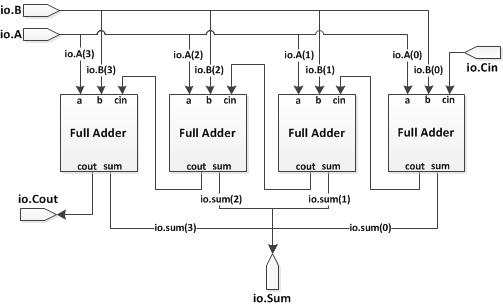
\includegraphics[width=80mm]{figs/4_Bit_Adder.jpg}
\caption{Block Diagram of 4-Bit Adder}
\label{overflow}
\end{figure}

\begin{scala}
// A 4-bit adder with carry in and carry out
class Adder4 extends Module {
  val io = new Bundle {
    val A    = UInt(INPUT, 4)
    val B    = UInt(INPUT, 4)
    val Cin  = UInt(INPUT, 1)
    val Sum  = UInt(OUTPUT, 4)
    val Cout = UInt(OUTPUT, 1)
  }
  // Adder for bit 0
  val Adder0 = Module(new FullAdder())
  Adder0.io.a   := io.A(0)
  Adder0.io.b   := io.B(0)
  Adder0.io.cin := io.Cin
  val s0 = Adder0.io.sum
  // Adder for bit 1
  val Adder1 = Module(new FullAdder())
  Adder1.io.a   := io.A(1)
  Adder1.io.b   := io.B(1)
  Adder1.io.cin := Adder0.io.cout
  val s1 = Cat(Adder1.io.sum, s0)
  // Adder for bit 2
  val Adder2 = Module(new FullAdder())
  Adder2.io.a   := io.A(2)
  Adder2.io.b   := io.B(2)
  Adder2.io.cin := Adder1.io.cout
  val s2 = Cat(Adder2.io.sum, s1)
  // Adder for bit 3
  val Adder3 = Module(new FullAdder())
  Adder3.io.a   := io.A(3)
  Adder3.io.b   := io.B(3)
  Adder3.io.cin := Adder2.io.cout
  io.Sum  := Cat(Adder3.io.sum, s2).toUInt()
  io.Cout := Adder3.io.cout
}
\end{scala}

In this example, notice how when referencing each module I/O we must first reference the \verb+io+ that contains the ports for the I/Os. Again, note how all assignments to the module I/Os use a reassignment operator \verb+:=+. When instantiating modules, it is important to make sure that you connect all the input and output ports. If a port is not connected, the Chisel compiler may optimize away portions of your design that it find unecessary due to the unconnected ports and throw errors or warnings.

\section{The Vec Class}

The \verb+Vec+ class allows you to create an indexable vector in Chisel which can be filled with any expression that returns a chisel data type. The general syntax for a \verb+Vec+ declaration is given by:
\begin{scala}
val myVec = 
  Vec.fill( <number of elements> ) { <data type> }
\end{scala}
Where \verb+<number of elements>+ corresponds to how long the vector is and \verb+<data type>+ corresponds to what type of class the vector contains.

For instance, if we wanted to instantiate a 10 entry vector of 5 bit UInt values, we would use:

\begin{scala}
val ufix5_vec10 := Vec.fill(10) { UInt(width = 5) }
\end{scala}

If we want to define a vector of registers...

\begin{scala}
val reg_vec32 := Vec.fill(32){ Reg() }
\end{scala}

In order to assign to a particular value of the \verb+Vec+, we simply assign the target value to the vector at a specified index. For instance, if we wanted to assign a UInt value of zero to the first register in the above example, the assignment would look like:

\begin{scala}
reg_vec32(1) := UInt(0)
\end{scala}

To access a particular element in the vector at some index, we specify the index of the vector. For example, to extract the 5th element of the register vector in the above example and assign it to some value \verb+reg5+, the assignment would look like:

\begin{scala}
val reg5 = reg_vec(5)
\end{scala}

The syntax for the \verb+Vec+ class is slightly different when instantiating a vector of modules. When instantiating a vector of modules the data type that is specified in the {} braces is slightly different than the usualy primitive types. To specify a vector of modules, we use the \verb+io+ bundle when specifying the type of the vector. For example, in order to specify a \verb+Vec+ with 16 modules , say \verb+FullAdder+s in this case, we would use the following declaration:

\begin{scala}
val FullAdders = 
  Vec.fill(16){ Module(new FullAdder()).io }
\end{scala}

Notice we use the keyword \verb+new+ in the vector definition before the module name \verb+FullAdder+. For how to actually access the \verb+io+ on the vector modules, refer to the next section.

\subsection{\problem{Vec Shift Reg}}

The next assignment is to construct a simple bit shift register.
The following is a the template from \verb+$TUT_DIR/problems/VecShiftRegisterSimple.scala+:

\begin{scala}
class VecShiftRegisterSimple extends Module {
  val io = new Bundle {
    val in  = UInt(INPUT,  8)
    val out = UInt(OUTPUT, 8)
  }
  val delays = Vec.fill(4){ Reg(UInt(width = 8)) }
  ...
  io.out := UInt(0)
}
\end{scala}

\noindent
where \verb+out+ is a four cycle delayed copy of values on \verb+in+.

\section{Parametrization}

In the previous Adder example, we explicitly instantiated four different copies of a \verb+FullAdder+ and wired up the ports. But suppose we want to generalize this structure to an n-bit adder. Like Verilog, Chisel allows you to pass parameters to specify certain aspects of your design. In order to do this, we add a parameter in the Module declaration to our Chisel definition.
For a carry ripple adder, we would like to parametrize the width to some integer value \verb+n+ as shown in the following example:

\begin{scala}

// A n-bit adder with carry in and carry out
class Adder(n: Int) extends Module {
  val io = new Bundle {
    val A    = UInt(INPUT, n)
    val B    = UInt(INPUT, n)
    val Cin  = UInt(INPUT, 1)
    val Sum  = UInt(OUTPUT, n)
    val Cout = UInt(OUTPUT, 1)
  }
  // create a vector of FullAdders
  val FAs = Vec.fill(n){ Module(new FullAdder()).io }

  // define carry and sum wires
  val carry = Vec.fill(n+1){ UInt(width = 1) }
  val sum   = Vec.fill(n){ Bool() } 

  // first carry is the top level carry in
  carry(0) := io.Cin

  // wire up the ports of the full adders
  for(i <- 0 until n) {
     FAs(i).a   := io.A(i)
     FAs(i).b   := io.B(i)
     FAs(i).cin := carry(i)
     carry(i+1) := FAs(i).cout
     sum(i)     := FAs(i).sum.toBool()
  }
  io.Sum  := sum.toBits().toUInt()
  io.Cout := carry(n)
}

\end{scala}

Note that in this example, we keep track of the sum output in a \verb+Vec+ of \verb+Bool+s. This is because Chisel does not support bit assignment directly. Thus in order to get the n-bit wide \verb+sum+ in the above example, we use an n-bit wide \verb+Vec+ of \verb+Bool+s and then cast it to a UInt(). Note that it must first be casted to the \verb+Bits()+ type before casting it to \verb+UInt()+.

You will notice that modules are instantiated in a Vec class which allows us to iterate through each module when assigning the ports connections to each \verb+FullAdder+. This is similar to the generate statement in Verilog. However, you will see in more advanced tutorials that Chisel can offer more powerful variations.

Instantiating a parametrized module is very similar to instantiating an unparametrized module except that we must provide arguments for the parameter values. For instance, if we wanted to instantiate a 4-bit version of the \verb+Adder+ module we defined above, it would look like:

\begin{scala}
val adder4 = Module(new Adder(4))
\end{scala}

We can also instantiate the \verb+Adder+ by explicitly specifying the value of it parameter \verb+n+ like the this:

\begin{scala}
val adder4 = Module(new Adder(n = 4))
\end{scala}

Explicitly specifying the parameter is useful when you have a module with multiple parameters. Suppose you have a parametrized FIFO module with the following module definition:

\begin{scala}
class FIFO(width: Int, depth: Int) extends Module {...}
\end{scala}

You can explicitly specify the parameter values in any order:

\begin{scala}
val fifo1 = Module(new FIFO(16, 32))
val fifo2 = Module(new FIFO(width = 16, depth = 32))
val fifo3 = Module(new FIFO(depth = 32, width = 16))
\end{scala}

All of the above definitions pass the same parameters to the FIFO module. Notice that when you explicitly assign the parameter values, they can occur in any order you want such as the definition for fifo3.

\section{Advanced Parametrization}

Although parameters can be passed explicitly through a Module's constructor, this technique does not scale when parameterizing large designs with many generic components. For a more detailed explanation of why a better parameterization method is needed, please see the Advanced Parameterization Manual. In addition, this manual explains heuristics for how to organize and parameterize large designs, which we highly recommend one reads prior to using this functionality in a design. The following, however, is a basic introduction.

Every Module has its own \verb+params+ object, which acts as a dictionary. Querying this object is shown below.

\begin{scala}
val width = params[Int]('width')
\end{scala}

If \verb+params+ is queried and no parameter matches the query, Chisel throws a \verb+ParameterUndefinedException+. Notice the query return type must be provided.

When a parent Module creates a child Module, the parent's \verb+params+ object is automatically cloned and passed to the child. In the following example, suppose the parent's params object returns \verb+10+ when queried for width. Because the \verb+Parent+ \verb+params+ object is automatically cloned for \verb+Child+, the \verb+Child+ query also returns \verb+10+.

\begin{scala}
class Parent extends Module {
  val io = new Bundle { ... }
  val width = params[Int]('width') // returns 10
  // create child Module implicitly passing params
  val child = Module(new Child) 
}
class Child extends Module {
  val io = new Bundle { ... }
  val width = params[Int]('width') // returns 10
}
\end{scala}

Suppose a parent Module wants to override or add parameters to its child's \verb+params+ object. This case requires adding a partial function (a Scala way of defining key-value mappings) to the \verb+Child+ Module constructor:

\begin{scala}
class Parent extends Module {
  val io = new Bundle { ... }
  val width = params[Int]('width') // returns 10
  val n = params[Int]('n') // returns 20
  // Partial function is added to Module constructor
  val child = Module(new Child,{'n' => 40})
}
class Child extends Module {
  val io = new Bundle { ... }
  val width = params[Int]('width') // returns 10
  val n = params[Int]('n') // returns 40
}
\end{scala}

An example which is impossible to do with simple parameterization, but simple with the advanced parameterization, is when using a generic \verb+Mesh+ generator with a custom \verb+MyRouter+ Module. The existing source code might look like:

\begin{scala}
class Mesh(routerConstructor: () => Router, n:Int) extends Module {
  val io = new Bundle { ... }
  val routers = Vec.fill(n){Module(routerConstructor())}
  hookUpRouters(routers)
}
\end{scala}

However, our custom \verb+MyRouter+ Module requires a parameter, \verb+RoutingFunction+ that we want to sweep for a design space evaluation. Using the simple parameterization method would require a change to the \verb+Mesh+ Module's constructor to include \verb+RoutingFunction+. 

Alternatively, one can use the \verb+params+ object to implicitly pass the \verb+RoutingFunction+:

\begin{scala}
class MyRouter extends Module {
  val io = new Bundle { ... }
  val myRoutingFunction = params[RoutingFunction]('r')
  ...
}
class Top extends Module {
  val io = new Bundle { ... }
  val mesh = Module(new Mesh(() => new MyRouter),{'r' => new RoutingFunction})
}
\end{scala}

For more advanced uses, tips, and tricks, please see the Advanced Parameterization Manual, in the documentation section of the website or the doc/parameters directory of the git repo. This is an evolving area and the documentation may not be as up-to-date as the code.

\section{Built In Primitives}

Like other HDL, Chisel provides some very basic primitives. These are constructs that are built in to the Chisel compiler and come for free. The Reg, UInt, and Bundle classes are such primitives that has already been covered. Unlike Module instantiations, primitive do not require explicit connections of their io ports to use. Other useful primitive types include the Mem and Vec classes which will be discussed in a more advanced tutorial. In this tutorial we explore the use of the \verb+Mux+ primitive

\subsection{The Mux Class}

The \verb+Mux+ primitive is a two input multiplexer. In order to use the \verb+Mux+ we first need to define the expected syntax of the \verb+Mux+ class. As with any two input multiplexer, it takes three inputs and one output. Two of the inputs correspond to the data values \verb+A+ and \verb+B+ that we would like to select which can be any width and data type as long as they are the same. The third input \verb+select+ which is a Bool type determines which one to output.
A \verb+select+ value of \verb+true+ will output the first value \verb+A+, while a \verb+select+ value of \verb+false+ will pass \verb+B+.

\begin{scala}
val out = Mux(select, A, B)
\end{scala}

Thus if \verb+A=10+, \verb+B=14+, and \verb+select+ was \verb+true+, the value of \verb+out+ would be assigned 10. Notice how using the \verb+Mux+ primitive type abstracts away the logic structures required if we had wanted to implement the multiplexer explicitly.

\subsection{\problem{Parameterized Width Adder}}

The next assignment is to construct an adder with a parameterized width and using the built in addition operator \verb!+!.
The following is a the template from \verb+$TUT_DIR/problems/Adder.scala+:

\begin{scala}
class Adder(val w: Int) extends Module {
  val io = new Bundle {
    val in0 = UInt(INPUT,  1)
    val in1 = UInt(INPUT,  1)
    val out = UInt(OUTPUT, 1)
  }
  ...
  io.out := UInt(0)
}
\end{scala}

\noindent
where \verb+out+ is sum of \verb+w+ width unsigned inputs \verb+in0+ and \verb+in1+.  
Notice how \verb+val+ is added to the width parameter value to 
allow the width to be accessible from the tester as a field of the adder module object.  Run 

\begin{bash}
make Adder.out
\end{bash}

\noindent 
until your circuit passes the tests.

% Martin: I would drop the following as it is just confusing in a tutorial
% state simple that there is a Mux primitive and that is fine.

%The instantiation would look something like this:
%
%\begin{scala}
%// where n is the width of A and m is the width of B
%val mux = Module(new Mux(n, m))
%mux.io.select := select
%mux.io.A      := A
%mux.io.B      := B
%val out = mux.io.out
%\end{scala}
%
%We see that clearly it is much cleaner to use the primitive \verb+Mux+ type instead of trying to write and implement our own general multiplexer since the \verb+Mux+ type does all the wiring for you.


%\section{Exercises}
%
%\subsection{n-bit Subtractor}
%
%Earlier in this tutorial we demonstarted how to parametrize and instantiate an n-bit ripple adder. <Finish this>
%


\chapter{Writing Scala Testbenches}
\section{The Scala Testbench Simulation}

Chisel's Scala based testbench is the first line of defense against simple bugs in your design. The Scala testbench uses several unique Chisel constructs to perform this. To see how this works, let's first explore a simple example.

\subsection{Scala Testbench Example}

Below is the \verb+ByteSelector.scala+ module definition from the previous tutorial and the corresponding Chisel test harness.

\begin{scala}
package TutorialExamples

import Chisel._

class ByteSelector extends Module {
  val io = new Bundle {
    val in     = UInt(INPUT, 32)
    val offset = UInt(INPUT, 2)
    val out    = UInt(OUTPUT, 8)
  }
  io.out := UInt(0, width = 8)
  when (io.offset === UInt(0)) {
    io.out := io.in(7,0)
  } .elsewhen (io.offset === UInt(1)) {
    io.out := io.in(15,8)
  } .elsewhen (io.offset === UInt(2)) {
    io.out := io.in(23,16)
  } .otherwise {
    io.out := io.in(31,24)
  }    
}

class ByteSelectorTests(c: ByteSelector) 
    extends Tester(c) {
  val test_in = 12345678
  for (t <- 0 until 4) {
    poke(c.io.in,     test_in)
    poke(c.io.offset, t)
    step(1)
    expect(c.io.out, (test_in >> (t * 8)) & 0xFF)
  }
}
\end{scala}

In the test harness \verb+ByteSelectorTests+ we see that the test portion is written in Scala with some Chisel constructs inside a \verb+Tester+ class definition. The device under test is passed to us as a parameter \verb+c+. 

In the \verb+for+ loop, the assignments for each input of the \verb+ByteSelector+ is set to the appropriate values using \verb+poke+. For this particular example, we are testing the \verb+ByteSelector+ by hardcoding the input to some known value and checking if each of the 4 offsets returns the appropriate byte. To do this, on each iteration we generate appropriate inputs to the module and tell the simulation to assign this value to the input of the device we are testing \verb+c+:

\begin{scala}
val test_in = 12345678
for (t <- 0 until 4) {
  // set in of the DUT to be some known word
  poke(c.io.in,     test_in)
  // set the offset of the DUT
  poke(c.io.offset, t)
  ...
}
\end{scala}

Next we step the circuit.  We next advance the simulation by calling the \verb+step+ function. This effectively advances the simulation one clock cycle in the presence of sequential logic. 

\begin{scala}
step(1)
\end{scala}

Finally, we check for expected outputs.
In this case, we check the expected output of \verb+ByteSelector+ as follows:

\begin{scala}
expect(c.io.out, (test_in >> (t * 8)) & 0xFF)
\end{scala}

This defines the reference output expected for this particular cycle of the simulation. Since the circuit we are testing is purely combinational, we expected that the output we define appears on any advancement of the simulation.  The \verb+expect+ function will record either true or false after checking if the output generates the expected reference output. The results of successive \verb+expect+'s are anded into a \verb+Tester+ field called \verb+ok+ which starts out as \verb+true+.  The value of the \verb+ok+ field determines the success or failure of the tester execution.

Actually \verb+expect+ is defined in terms of \verb+peek+ roughly as follows:

\begin{scala}
def expect (data: Bits, expected: BigInt) = 
  ok = peek(data) == expected && ok
\end{scala}

where \verb+peek+ gets the value of a signal from the DUT.

\subsection{Simulation Debug Output}

Now suppose we run the testbench for the \verb+ByteSelector+ defined previously. To do this, \verb+cd+ into the \verb+$DIR/problems+ directory and run \verb+make ByteSelector+.

When we run the testbench, we will notice that the simulation produces debug output every time the \verb+step+ function is called. Each of these calls gives the state of the inputs and outputs to the \verb+ByteSelector+ and whether the check between the reference output and expected output matched as shown below:

\begin{bash}
STARTING ../emulator/problems/ByteSelector
---
POKE ByteSelector__io_in <- 12345678
POKE ByteSelector__io_offset <- 0
STEP 1 <- 0
PEEK ByteSelector__io_out -> 0x4e
EXPECT ByteSelector__io_out <- 78 == 78 PASS
POKE ByteSelector__io_in <- 12345678
POKE ByteSelector__io_offset <- 1
STEP 1 <- 0
PEEK ByteSelector__io_out -> 0x61
EXPECT ByteSelector__io_out <- 97 == 97 PASS
...
POKE ByteSelector__io_in <- 12345678
POKE ByteSelector__io_offset <- 3
STEP 1 <- 0
PEEK ByteSelector__io_out -> 0x00
EXPECT ByteSelector__io_out <- 0 == 0 PASS
PASSED   // Final pass assertion
[success] Total time: 6 s, completed Feb 23, 2014 9:52:22 PM
\end{bash}

Also notice that there is a final pass assertion "PASSED" at the end which corresponds to the \verb+allGood+ at the very end of the testbench. In this case, we know that the test passed since the allGood assertion resulted in a "PASSED". In the event of a failure, the assertion would result in a "FAILED" output message here.

\subsection{General Testbench}

In general, the scala testbench should have the following rough structure:

\begin{itemize}
\item Set inputs using \verb+poke+
\item Advance simulation using \verb+step+
\item Check expected values using \verb+expect+ (and/or \verb+peek+)
\item Repeat until all appropriate test cases verified
\end{itemize}

For sequential modules we may want to delay the output definition to the appropriate time as the \verb+step+ function implicitly advances the clock one period in the simulation. Unlike Verilog, you do not need to explicitly specify the timing advances of the simulation; Chisel will take care of these details for you.

\section{\problem{Max2 Testbench}}

In this assignment, write a tester for the \verb+Max2+ circuit:

\begin{scala}
class Max2 extends Module {
  val io = new Bundle {
    val in0 = UInt(INPUT,  8)
    val in1 = UInt(INPUT,  8)
    val out = UInt(OUTPUT, 8)
  }
  io.out := Mux(io.in0 > io.in0, io.in0, io.in1)
}
\end{scala}

\noindent
found in \verb+$TUT_DIR/problems/Max2.scala+ by filling in the following tester:

\begin{scala}
class Max2Tests(c: Max2) extends Tester(c) {
  for (i <- 0 until 10) {
    // FILL THIS IN HERE
    poke(c.io.in0, 0)
    poke(c.io.in1, 0)
    // FILL THIS IN HERE
    step(1)
    expect(c.io.out, 1)
  }
}
\end{scala}

\noindent 
using random integers generated as follows:

\begin{scala}
// returns random int in 0..lim-1
val in0 = rnd.nextInt(lim) 
\end{scala}

\noindent
Run 

\begin{bash}
make Max2.out
\end{bash}

\noindent 
until the circuit passes your tests.

\section{Limitations of the Testbench}

The Chisel testbench works well for simple tests and small numbers of simulation iterations. However, for larger test cases, the Chisel testbench quickly becomes more complicated and slower simply due to the inefficiency of the infrastructure. For these larger and more complex test cases, we recommend using the C++ emulator or Verilog test harnesses which run faster and can handle more rigorous test cases.



\chapter{Creating Your Own Project}
\section{Creating Your Own Projects}

In order to create your own projects from scratch, you will need to create a directory, a Chisel source file, and a build.sbt configuration file. In the first part of this tutorial we cover the basic calls to SBT in order generate appropriate files. At the end of the tutorial, we will explain how the Makefile infrastructure can make the process more streamlined.

\subsection{Directory Structure}

The simplest project file organization is using a single directory containing your Scala project file and your Chisel source file.  The project directory structure would look like:

\begin{bash}
Hello/
  build.sbt   # scala configuration file
  Hello.scala # your source file
\end{bash}

We will refer to the path to the \verb+Hello+ directory as \verb+$BASEDIR+ from here on.  More sophisticated directory structures can be useful in the future.  Consult the SBT documentation for more information.

\subsection{The Source Directory and Chisel Main}

The top directory \verb+$BASEDIR/+ contains Scala source files containing all of the Chisel module definitions for your circuit and a main method.  In this simple example, we have one Scala source file as shown below:

\begin{scala}
package Hello

import Chisel._

class HelloModule extends Module {
  val io = new Bundle { 
    val out = UInt(OUTPUT, 8)
  }
  io.out := UInt(42)
}

class HelloModuleTests(c: HelloModule) 
    extends Tester(c) {
  step(1)
  expect(c.io.out, 42)
}

object hello {
  def main(args: Array[String]): Unit = {
    val margs = 
      Array("--backend", "c", "--genHarness", "--compile", "--test")
    chiselMainTest(margs, () => Module(new HelloModule())) {
        c => new HelloModuleTests(c)
      })
  }
}
\end{scala}

In the above example, we have a module definition in package \verb+Hello+ for a \verb+Hello+ module. The main method calls \verb+chiselMainTest+ for a new Hello module\footnote{Note that when you have multiple Scala files, in order for main to recognize your module definition, your module definition must be in the same package as the main function}. In addition to creating the module, the call to \verb+chiselMainTest+ also includes a call to execute the scala testbench defined in the routine \verb+HelloModuleTests+.

\subsection{The build.sbt Template}

The \verb+build.sbt+ configuration file is located in the top folder and contains a number of settings used by \verb+sbt+ when building and compiling the Chisel sources.  The following shows the recommended \verb+build.sbt+ template that should be used:

\begin{scala}
scalaVersion := "2.10.2"

resolvers ++= Seq(
  "scct-github-repository" at "http://mtkopone.github.com/scct/maven-repo"
)

libraryDependencies += 
  "edu.berkeley.cs" %% "chisel" % "latest.release"
\end{scala}

The SBT project file contains a reference to Scala version greater or equal to 2.10.2 and a dependency on the latest release of the Chisel library.

\section{Compiling the Chisel Source}

\subsection{Compiling the Emulation Files}

In order to launch SBT to compile the Chisel code we must first be in the directory \verb+$BASEDIR/+. The following call is then made to compile and run the Hello module:

\begin{bash}
sbt run
\end{bash}

\subsection{Running the Chisel Tests}

To actually run the tests referenced in the main method of \verb+$BASEDIR/Hello.scala+, we need to tell SBT to also generate the harness and run the tests. For instance, for our Hello module introduced earlier, the Chisel main method references a test routine \verb+HelloTests+. In order to both compile the Hello component and run the tests defined in \verb+Hello+, we make the following call to sbt:

\begin{bash}
sbt "run --backend c --compile --test --genHarness"
\end{bash}

Note the addition of the 5 arguments at the end of the call to \verb+run+. This will both compile the \verb+.cpp+ and \verb+.h+ files for the emulator and run the Chisel tests defined. 

\subsection{Compiling Verilog}

Similarly to compile the Chisel code and generate the Verilog HDL, a similar call to SBT is made with slightly different arguments. The call looks like:

\begin{bash}
sbt "run --backend v --genHarness"
\end{bash}

Notice the call is very similar to when generating C++; the key difference is the parameter to the \verb+--backend+ attribute which is now \verb+v+ which specifies to sbt that we would like to compile our Chisel component to Verilog. 

\section{Putting It All Together}

In summary, the bare minimum project components that are necessary for your project to get off the ground are the following files:

\begin{enumerate}
\item \verb+$BASEDIR/build.sbt+
\item \verb+$BASEDIR/<Chisel source files>.scala+
\end{enumerate}

Together, these files compose a Chisel project and can be used to generate the Verilog and C++ files. It is strongly recommended that you supplement the file structure with appropriate Makefiles but is not strictly necessary (examples can be found in the Chisel tutorial project).



\chapter{Conditional Assignments and Memories}
\section{Conditional Register Updates}

As shown earlier in the tutorial, conditional register updates are performed with the \verb+when+ block which takes a \verb+Bool+ value or some boolean expression to evaluate.
In this section we more fully explore how to use this \verb+when+ conditional update structure.

If a \verb+when+ block is used by itself, Chisel will assume that if the condition for the \verb+when+ block doesn't evaluate to true, there is no update to the register value. However, most of the time we don't want to limit ourselves to a single conditional. Thus in Chisel we use \verb+.elsewhen+ and \verb+.otherwise+ statements to select between multiple possible register updates as shown in the following sections.

\subsection{The .elsewhen Clause}

When specifying a conditional update, we may want to check several conditions which we want to check in some order. 
To do this for register updates, we use a \verb+when ... .elsewhen+ structure. This is analagous to an \verb+if... else if+ control structure in sequential programming. \footnote{Note that the if .. else if control structure in Chisel is NOT used to specify register updates} 
As with \verb+else if+ clauses, as many \verb+.elsewhen+ statements can be chained together in a single \verb+when+ block. 

The general structure thus looks like:

%$when$ (<condition 1>) {<register update 1>}
%.elsewhen (<condition 2>) {<register update 2>}
%...
%.elsewhen (<condition N>) {<register update 3>}

\begin{scala}
when (<condition 1>) {<register update 1>}
.elsewhen (<condition 2>) {<register update 2>}
...
.elsewhen (<condition N>) {<register update N>}
\end{scala}

Where \verb+<condition 1>+ through \verb+<condition N>+ represent the trigger conditions of their respective \verb+<register update>+ segments.

An example of this statement in action is shown in the following implementation of a simple stack pointer. Suppose, we need to maintain a pointer that keeps track of the address of the top of a stack. Given a signal \verb+pop+ that decrements the stack pointer address by 1 entry and a signal \verb+push+ that increments the stack pointer address by 1 entry, the implementation of just the pointer would look like the following:

\begin{scala}
class StackPointer(depth:Int) extends Module {
  val io = new Bundle {
    val push = Bool(INPUT)
    val en   = Bool(INPUT)
    val pop  = Bool(INPUT)
  }

  val sp = Reg(init = UInt(0, width = log2Up(depth)))
  
  when (io.en && io.push && (sp != UInt(depth-1))) {
    sp := sp + UInt(1)
  } .elsewhen(io.en && io.pop && (sp > UInt(0))) {
    sp := sp - UInt(1)
  }
}
\end{scala}

Notice that in this implementation, the push signal has higher priority over the pop signal as it appears earlier in the \verb+when+ block.

\subsection{The .otherwise Clause}

In order to specify a default register update value if all the conditions in the \verb+when+ block fail to trigger, we use an \verb+.otherwise+ clause. 
The \verb+.otherwise+ clause is analagous to the \verb+else+ case that completes an \verb+if ... else+ block. The \verb+.otherwise+ statement must occur last in the \verb+when+ block.

The general structure for the complete \verb+when+ block now looks like:
\begin{scala}
when (<condition 1>) {<register update 1>}
.elsewhen (<condition 2>) {<register update 2>}
...
.elsewhen (<condition N>) {<register update N>}
.otherwise {<default register update>}
\end{scala}

In the previous example, we could add a default statement which just assigns \verb+sp+ to the current value of \verb+sp+. The \verb+block+ would then look like:

\begin{scala}
when(io.en && io.push && (sp != UInt(depth-1))) {
  sp := sp + UInt(1)
} .elsewhen(io.en && io.pop && (sp > UInt(0))) {
  sp := sp - UInt(1)
} .otherwise {
  sp := sp
}
\end{scala}

The explicit assignment to preserve the value of \verb+sp+ is redundant in this case but it captures the point of the \verb+.otherwise+ statement.

\subsection{The unless Clause}

% Martin: this feels a little bit strange as it is not a usual construct in a programming language.
% It is simple !condition, right? So I would drop it.

To complement the \verb+when+ statement, Chisel also supports an \verb+unless+ statement. The \verb+unless+ statement is a conditional assignment that triggers only if the condition is false. The general structure for the \verb+unless+ statement is:

\begin{scala}
unless ( <condition> ) { <assignments> }
\end{scala}

For example, suppose we want to do a simple search of the contents of memory and determine the address that contains some number. Since we don't know how long the search will take, the module will output a \verb+done+ signal when it is finished and until then, we want to continue to search memory. The Chisel code for the module would look like:

\begin{scala}
class MemorySearch extends Module {
  val io = new Bundle {
    val target  = UInt(INPUT,  4)
    val address = UInt(OUTPUT, 3)
    val en      = Bool(INPUT)
    val done    = Bool(INPUT)
  }
  val index  = Reg(init = UInt(0, width = 3))
  val list   = Vec(UInt(0), UInt(4), UInt(15), UInt(14), UInt(2), UInt(5), UInt(13))
  val memVal = list(index)

  val done = (memVal === io.target) || (index === UInt(7))

  unless (done) {
    index := index + UInt(1)
  }
  io.done    := done
  io.address := index
}
\end{scala}

In this example, we limit the size of the memory to 8 entries and use a vector of literals to create a read only memory. Notice that the \verb+unless+ statement is used to terminate the iteration if it see that the \verb+done+ signal is asserted. Otherwise, it will continue to increment the index in memory until it finds the value in \verb+target+ or reaches the last index in the memory (7).

\section{Combinational Conditional Assignment}

You can also use the \verb+when .elsewhen .otherwise+ block to define combinational values that may take many values. For example, the following Chisel code show how to implement a basic arithmetic unit with 4 operations: add, subtract, and pass. In this example, we check the opcode to determine which operation to perform and conditionally assign the output.

\begin{scala}
class BasicALU extends Module {
  val io = new Bundle {
    val a      = UInt(INPUT, 4)
    val b      = UInt(INPUT, 4)
    val opcode = UInt(INPUT, 2)
    val output = UInt(OUTPUT, 4)
  }
  io.output := UInt(0) 
  when (io.opcode === UInt(0)) {
    io.output := io.a + io.b   // ADD
  } .elsewhen (io.opcode === UInt(1)) {
    io.output := io.b - io.b   // SUB
  } .elsewhen (io.opcode === UInt(2)) {
    io.output := io.a  	       // PASS A
  } .otherwise {
    io.output := io.b          // PASS B
  }
}
\end{scala}

Notice that this can easily be easily expanded to check many different conditions for more complicated arithmetic units or combinational blocks.

\section{Read Only Memories}

To instantiate read only memories in Chisel, we use a vector of constant literals and specify a literal type. For example, in order to instantiate an 4 entry read only memory with the values 0 to 3, the definition would look like the following:

\begin{footnotesize}
\begin{scala}
val numbers = 
  Vec(UInt(0),UInt(1),UInt(2),UInt(3)){ UInt(width = 2) }
\end{scala}
\end{footnotesize}

Notice that we need to specify the type of literal in the {...} braces following the literals. Accessing the values in the read only memory is the same as accessing an entry in a \verb+Vec+. For example, to access the 2nd entry of the memory we would use:

\begin{scala}
val entry2 = numbers(2)
\end{scala}

\section{Read-Write Memories}

Chisel contains a primitive for memories called \verb+Mem+. Using the \verb+Mem+ class it is possible to construct multi-ported memory that can be synchronous or combinational read. \footnote{The complete definition can be found in the chisel source in  Mem.scala}

\subsection{Basic Instantiation}

The \verb+Mem+ construction takes a memory depth and a data type which it is composed of. The general declaration structure looks like:

\begin{scala}
val myMem = Mem(<type>, <depth>)
\end{scala}

Where \verb+<depth>+ corresponds to the number of entries of \verb+<type>+ are in the memory.

For instance, if you wanted to create a 128 deep memory of 32 bit UInt types, you would use the following instantiation:

\begin{scala}
val myMem = Mem(UInt(width = 32), depth = 128)
\end{scala}

Note that when constructing a memory in Chisel, the initial value of memory contents cannot be specified. Therefore, you should never assume anything about the initial contents of your \verb+Mem+ class.

\subsection{Synchronous vs. Combinational Read}

It is possible to specify either combinational or synchronous read behavior during instantiation by setting the \verb+seqRead+ parameter when defining the \verb+Mem+. The \verb+seqRead+ parameter is a \verb+Bool+ that tells Chisel if you want synchronous read behavior memory or not.

For instance, if we wanted a combinational read 128 entry memory of 32 bit UInt types, we would use the following definition:

\begin{scala}
val asyncMem = 
  Mem(UInt(width = 32), 128, seqRead = false)
\end{scala}

Likewise, if we wanted a synchronous read 128 entry memory of 32 bit UInt types, we would set the \verb+seqRead+ to true:

\begin{scala}
val syncMem = 
  Mem(UInt(width = 32), 128, seqRead = true)
\end{scala}

% this needs more elaboration. Memories in hardware are tough...

By default, Chisel will assume that the read behavior is combinational.

\subsection{Adding Write Ports}

To add write ports to the \verb+Mem+, we use a \verb+when+ block to allow Chisel to infer a write port. Inside the \verb+when+ block, we specify the location and data for the write transaction. In general, adding a write port requires the following definition:

\begin{scala}
when (<write condition> ) {
  <memory name>( <write address> ) := <write data>
}
\end{scala}

Where \verb+<write address>+ refers to the entry number in the memory to write to. Also notice that we use the reassignment operator \verb+:=+ when writing to the memory. 


For example, suppose we have a 128 deep memory of 32 bit UInt types. If we wanted to write a 32 bit value \verb+dataIn+ to the memory at location \verb+writeAddr+ if as write enable signal \verb+we+ is true, our Chisel code would look like:

\begin{scala}
...
val myMem = Mem(UInt(width = 32), depth = 128)
when (wen) {
  myMem(writeAddr) := dataIn
}
...
\end{scala}

<what is the behavior of multiple write ports?>

\subsection{Adding Read Ports}

Depending on the type of read behaviour specified, the syntax for adding read ports to \verb+Mem+ in Chisel is slightly different for combinational read and synchronous read memories.

\subsubsection{Combinational Read Ports}

For combinational read memories, adding read ports to the memory simply amounts to placing an assignment inside a \verb+when+ block with some trigger condition. If you want Chisel to infer multiple read ports, simply add more assignments in the \verb+when+ definition. The general definition for read ports is thus:

\begin{scala}
when (<read condition>) {
  <read data 1> := <memory name>( <read address 1> )
  ...
  <read data N> := <memory name>( <read address N>)
}
\end{scala}

For instance, if you wanted a 128 entry memory of 32 bit UInt values with two combinational read ports, with some read enable \verb+re+ and reads from addresses \verb+raddr1+ and \verb+raddr2+, we would use the following \verb+when+ block definition:

\begin{scala}
...
val myMem = 
  Mem(UInt(width = 32), 128, seqRead = false)
val read_port1 = UInt(width = 32)
val read_port2 = UInt(width = 32)
when (re) {
  read_port1 := myMem(raddr1)
  read_port2 := myMem(raddr2)
}
...
\end{scala}

Note that the type and width of the \verb+read_port1+ and \verb+read_port2+ should match the type and width of the entries in the \verb+Mem+.

\subsubsection{Synchronous Read Ports}

In order to add synchronous read ports to the Chisel \verb+Mem+ class, Chisel requires that the output from the memory be assigned to a \verb+Reg+ type. Like the combinational read port, a synchronous read assignment must occur in a \verb+when+ block. The general structure for the definition of a synchronous read port is as follows:

\begin{scala}
...
val myMem = 
  Mem(UInt(width = 32), depth = 128, seqRead = true)
val read_port = Reg(UInt(width = 32))
when (re) {
  read_port := myMem(raddr)
}
...
\end{scala}

\subsection{Example of Mem in Action}

% Martin: no, it was not yet shown
%We introduced a basic stack pointer bookkeeping example earlier in the tutorial. In this section we show how the complete stack implementation would look like.

Here we provide a small example of using a memory by implementing a stack.

Suppose we would like to implement a stack that takes two signals \verb+push+ and \verb+pop+ where \verb+push+ tells the stack to push an input \verb+dataIn+ to the top of the stack, and \verb+pop+ tells the stack to pop off the top value from the stack. Furthermore, an enable signal \verb+en+ disables pushing or popping if not asserted. Finally, the stack should always output the top value of the stack.

\begin{scala}
class Stack(depth: Int) extends Module {
  val io = new Bundle {
    val dataIn  = UInt(INPUT,  32)
    val dataOut = UInt(OUTPUT, 32)
    val push    = Bool(INPUT)
    val pop     = Bool(INPUT)
    val en      = Bool(INPUT)
  }
  
  // declare the memory for the stack
  val stack_mem = 
    Mem(UInt(width = 32), depth, seqRead = false)
  val sp = Reg(init = UInt(0, width = log2Up(depth)))
  val dataOut = Reg(init = UInt(0, width = 32))
  
  // Push condition - make sure stack isn't full
  when(io.en && io.push && (sp != UInt(depth-1))) {
    stack_mem(sp + UInt(1)) := io.dataIn
    sp := sp + UInt(1)
  } 
  // Pop condition - make sure the stack isn't empty
  .elsewhen(io.en && io.pop && (sp > UInt(0))) {
    sp := sp - UInt(1)
  }
  
  when(io.en) {
    dataOut := stack_mem(sp)
  }

  io.dataOut := dataOut
}
\end{scala}

Since the module is parametrized to be \verb+depth+ entries deep, in order to correctly extract the minimum width of the stack pointer \verb+sp+ we take the \verb+log2Up(depth)+. This takes the base 2 logarithm of \verb+depth+ and rounds up.

\subsection{\problem{Load/Search Mem}}

In this assignment, write a memory module that supports loading elements and searching based on the following template:

\begin{scala}
class DynamicMemorySearch(val n: Int, val w: Int) extends Module {
  val io = new Bundle {
    val isWr   = Bool(INPUT)
    val wrAddr = UInt(INPUT,  log2Up(n))
    val data   = UInt(INPUT,  w)
    val en     = Bool(INPUT)
    val target = UInt(OUTPUT, log2Up(n))
    val done   = Bool(OUTPUT)
  }
  val index  = Reg(init = UInt(0, width = log2Up(n)))
  val memVal = UInt(0)
  /// fill in here
  io.done   := Bool(false)
  io.target := index
}
\end{scala}

\noindent
and found in \verb+$TUT_DIR/problems/DynamicMemorySearch.scala+.
Notice how it support depth and width parameters \verb+n+ and \verb+w+ and 
how the address width is computed from the depth. Run 

\begin{bash}
make DynamicMemorySearch.out
\end{bash}

\noindent 
until your circuit passes the tests.


\chapter{Scripting Hardware Generation}
\section{Using the For loop}

Often times parametrization requires instantiating multiple components which are connected in a very regular structure. A revisit to the parametrized \verb+Adder+ component definition shows the \verb+for+ loop construct in action:

\begin{scala}
// A n-bit adder with carry in and carry out
class Adder(n: Int) extends Module {
  val io = new Bundle {
    val A    = UInt(INPUT, n)
    val B    = UInt(INPUT, n)
    val Cin  = UInt(INPUT, 1)
    val Sum  = UInt(OUTPUT, n)
    val Cout = UInt(OUTPUT, 1)
  }
  // create a vector of FullAdders
  val FAs   = Vec.fill(n){ Module(new FullAdder()).io }
  val carry = Vec.fill(n+1){ UInt(width = 1) }
  val sum   = Vec.fill(n){ Bool() }

  // first carry is the top level carry in
  carry(0) := io.Cin

  // wire up the ports of the full adders
  for(i <- 0 until n) {
     FAs(i).a   := io.A(i)
     FAs(i).b   := io.B(i)
     FAs(i).cin := carry(i)
     carry(i+1) := FAs(i).cout
     sum(i)     := FAs(i).sum.toBool()
  }
  io.Sum  := sum.toBits().toUInt()
  io.Cout := carry(n)
}
\end{scala}

Notice that a Scala integer \verb+i+ value is used in the \verb+for+ loop definition as the index variable. This indexing variable is specified to take values from 0 \verb+until+ n, which means it takes values 0, 1, 2..., n-1. If we wanted it to take values from 0 to n inclusive, we would use \verb+for (i <- 0 to n)+.

It is also important to note, that the indexing variable \verb+i+ does not actually manifest itself in the generated hardware. It exclusively belongs to Scala and is only used in declaring how the connections are specified in the Chisel component definition.

The for loop construct is also very useful for assigning to arbitrarily long \verb+Vec+s 

\section{Using If, Else If, Else}

As previously mentioned, the \verb+if, elseif,+ and \verb+else+ keywords are reserved for Scala control structures. What this means for Chisel is that these constructs allow you to selectively generate different structures depending on parameters that are supplied. This is particularly useful when you want to turn certain features of your implementation "on" or "off", or if you want to use a different variant of some component.

For instance, suppose we have several simple counters that we would like to package up into a general purpose counter module: UpCounter, DownCounter, and OneHotCounter. From the definitions below, we notice that for these simple counters, the I/O interfaces and parameters are identical:

\begin{scala}
// Simple up counter that increments from 0 and wraps around
class UpCounter(CounterWidth:Int) extends Module {
  val io = new Bundle {
    val output = UInt(OUTPUT, CounterWidth)
    val ce     = Bool(INPUT)
  }...
}

// Simple down counter that decrements from 
// 2^CounterWidth-1 then wraps around
class DownCounter(CounterWidth:Int) extends Module{
  val io = new Bundle {
    val output = UInt(OUTPUT, CounterWidth)
    val ce     = Bool(INPUT)
  }...
}

// Simple one hot counter that increments from one hot 0 
// to CounterWidth-1 then wraps around
class OneHotCounter(CounterWidth:Int) extends Module {
  val io = new Bundle {
      val output = UInt(OUTPUT, CounterWidth)
      val ce     = Bool(INPUT)
  }...
}
\end{scala}

We could just instantiate all three of these counters and multiplex between them but if we needed one at any given time this would be a waste of hardware. In order to choose between which of these three counters we want to instantiate, we can use Scala's \verb+if, else if, else+ statements to tell Chisel how to pick which component to instantiate based on a \verb+CounterType+ parameter:

\begin{scala}
class Counter(CounterWidth: Int, CounterType: String) 
    extends Module {
  val io = new Bundle {
    val output = UInt(OUTPUT, CounterWidth)
    val ce     = Bool(INPUT)
  }
  if (CounterType == "UpCounter") {
     val upcounter = new UpCounter(CounterWidth)
     upcounter.io.ce := io.ce
     io.output := upcounter.io.output
  } else if (CounterType == "DownCounter") {
    val downcounter = new DownCounter(CounterWidth)
    downcounter.io.ce := io.ce
    io.output := downcounter.io.output
  } else if (CounterType == "OneHotCounter") {
    val onehotcounter = new OneHotCounter(CounterWidth)
    onehotcounter.io.ce := io.ce
    io.output := onehotcounter.io.output
  } else {
    // default output 1
    io.output := UInt(1)
  }
}
\end{scala}

By consolidating these three counter components into a single \verb+Counter+ module, we can instantiate a different counter by simply changing the parameter \verb+CounterType+. For instance:

\begin{scala}
// instantiate a down counter of width 16
val downcounter = 
  Module(new Counter(16, "DownCounter"))

// instantiate an up counter of width 16
val upcounter = 
  Module(new Counter(16, "UpCounter"))

// instantiate a one hot counter of width 16
val onehotcounter = 
  Module(new Counter(16, "OneHotCounter"))
\end{scala}

This allows seamless alternation between them.

\section{Using def}

Chisel also allows the usage of the Scala \verb+def+ statement to define Chisel code that may be used frequently. These \verb+def+ statements can be packaged into a Scala Object and then called inside a Module. The following Chisel code shows an alternate implementation of an counter using \verb+def+ that increments by \verb+amt+ if the \verb+inc+ signal is asserted.

\begin{scala} 
object Counter {
  def wrapAround(n: UInt, max: UInt) = 
    Mux(n > max, UInt(0), n)

  def counter(max: UInt, en: Bool, amt: UInt) = {
    val x = Reg(init = UInt(0, max.getWidth))
    x := wrapAround(x + amt, max)
    x
  }
}

class Counter extends Module {
  val io = new Bundle {
    val inc = Bool(INPUT)
    val amt = UInt(INPUT,  4)
    val tot = UInt(OUTPUT, 8)
  }
  io.tot := counter(UInt(255), io.inc, io.amt)
}
\end{scala}
 
\noindent
In this example, we use calls to subroutines defined in the \verb+Counter+ object in order to perform the appropriate logic. 

\section{\problem{Parameterized Vec Shift Reg}}

The next assignment is to construct a bit shift register with delay parameter.
The following is a the template from \verb+$TUT_DIR/problems/VecShiftRegisterParam.scala+:

\begin{scala}
class VecShiftRegisterParam(val n: Int, val w: Int) extends Module {
  val io = new Bundle {
    val in  = UInt(INPUT,  w)
    val out = UInt(OUTPUT, w)
  }
  ...
  io.out := UInt(0)
}
\end{scala}

\noindent
where \verb+out+ is a \verb+n+ cycle delayed copy of values on \verb+in+.  
Also notice how \verb+val+ is added to each parameter value to 
allow those values to be accessible from the tester. Run 

\begin{bash}
make VecShiftRegisterParam.out
\end{bash}

\noindent 
until your circuit passes the tests.

\section{\problem{Mul Lookup Table}}

The next assignment is to write a 16x16 multiplication table using \verb+Vec+.
The following is a the template from \verb+$TUT_DIR/problems/Mul.scala+:

\begin{scala}
class Mul extends Module {
  val io = new Bundle {
    val x   = UInt(INPUT,  4)
    val y   = UInt(INPUT,  4)
    val z   = UInt(OUTPUT, 8)
  }
  val muls = new ArrayBuffer[UInt]()

  // flush this out ...

  io.z := UInt(0)
}
\end{scala}

\noindent
As a hint build the lookup table using a rom constructed from the \verb+tab+ lookup table represented as a Scala ArrayBuffer with incrementally added elements (using \verb!+=!):

\begin{scala}
val tab = Vec(muls)
\end{scala}

\noindent
and lookup the result using an address formed from the \verb+x+ and \verb+y+ inputs as follows:

\begin{scala}
io.z := tab(Cat(io.x, io.y))
\end{scala}

\noindent
Run 

\begin{bash}
make Mul.out
\end{bash}

\noindent 
until your circuit passes the tests.

% The first call to \verb+counter+ in the \verb+Counter+ module


\end{document}
